\subsection{Architektura - GUI}\label{subsec:architektura-gui}

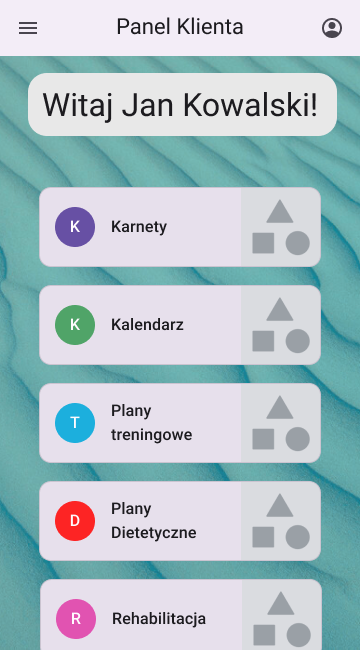
\includegraphics[width=0.5\textwidth]{latex/gui/main.png}

{Po zalogowaniu się do aplikacji, użytkownik jest witany na głównym ekranie, gdzie znajduje się menu nawigacyjne umożliwiające szybki dostęp do wszystkich dostępnych funkcji. Interfejs graficzny został zaprojektowany w sposób przyjazny dla użytkownika, z wykorzystaniem estetycznego i responsywnego designu, który sprawia, że korzystanie z aplikacji jest łatwe i intuicyjne.}

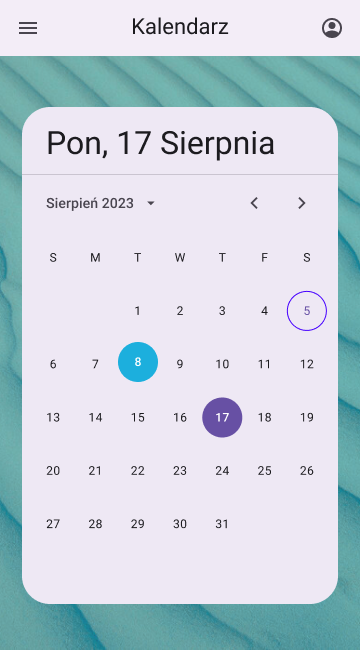
\includegraphics[width=0.5\textwidth]{latex/gui/calendar.png}

{Jednym z kolejnych ekranów do których może przejść użytkownik jest Kalendarz - miejsce w którym użytkownik może sprawdzić historię swoich treningów, zajęć grupowych, czy wizyt u dietetyków oraz rehabilitantów. Z poziomu kalendarza można również planować kolejne aktywności. Kalendarz automatycznie aktualizuje się w przypadku zapisania się na wizytę u specjalisty.}

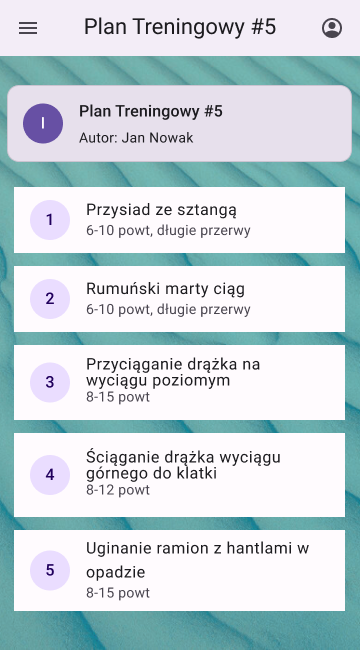
\includegraphics[width=0.5\textwidth]{latex/gui/training.png}

{Kolejnym kluczowym elementem aplikacji są treningi. Użytkownik po otrzymaniu planu treningowego może go wyświetlać na swoim koncie oraz przeglądać spersonalizowane uwagi przygotowane przez trenera personalnego.}

{Interfejs graficzny został zaprojektowany tak, aby był prosty i intuicyjny dla użytkowników o różnym poziomie doświadczenia. Wszystkie funkcje są łatwo dostępne i zorganizowane w przejrzysty sposób, co pozwala szybko odnaleźć potrzebne informacje i opcje.}

{Technologie wykorzystane przy implementacji GUI:
\begin{itemize}
    \item Aplikacje mobilne: język kotlin wraz z frameworkiem Jetpack Compose, który znacznie ułatwia pisanie interfejsów spełniających wszelkie normy dostępności
    \item Aplikacja webowa: react.js z wykorzystaniem frameworku Bootstrap
\end{itemize}
}
